%-*- ES -*-
%----------------------------------------------------------------------
% Capitulo: Implementacion de la solución propuesta
%----------------------------------------------------------------------

\section{Propuestas: Introducción}

Se han investigado tres alternativas enfocadas en redes internas para mejorar la seguridad de las 
mismas, luego de eso se eligió la que más ventajas nos ofreció.
Las alternativas son las siguientes: Los certificados auto-firmados (\emph{Self-signed Certificates}), implementar
una entidad certificante interna, y la utilización de un certificado emitido por una entidad
certificante conocida.

\section{Propuesta 1: Self-signed Certificates}

Un certificado autofirmado es un certificado digital que no está firmado por una 
autoridad de certificación (CA) de confianza pública (o privada). 
La razón por la que se consideran diferentes de los certificados tradicionales es que 
quien los crea, emite y firma es la empresa o el desarrollador responsable del sitio. 

Los certificados autofirmados son los menos útiles de los tres. Firefox facilita su uso 
de forma segura; crea una excepción en la primera visita, después de lo cual el 
certificado autofirmado se considera válido en las conexiones posteriores. Otros 
navegadores hacen que haga clic en una advertencia de certificado cada vez. A menos 
que esté comprobando la huella digital del certificado cada vez, no es posible hacer 
que ese certificado autofirmado sea seguro. Incluso con Firefox, puede resultar 
difícil utilizar estos certificados de forma segura.

\begin{center}
   \begin{figure}   
      \begin{center}
         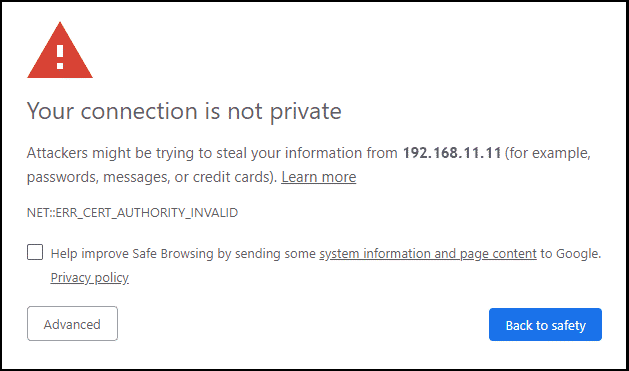
\includegraphics[width=13cm,height=8.2cm]{self-signed.png}
      \end{center}
      \caption{Advertencia Certificado Autofirmado}
   \end{figure}
\end{center}

Por ejemplo, para solicitar un certificado SSL de una CA de confianza como Verisign o 
GoDaddy, se debe enviar una Solicitud de firma de certificado (CSR) y te dan un 
certificado a cambio, que firmaron con su certificado raíz y clave privada. Todos 
los navegadores tienen una copia (o acceden a una copia desde el sistema operativo) 
del certificado raíz, por lo que el navegador puede verificar que su certificado 
fue firmado por una CA confiable.

En la infraestructura de clave pública (PKI), ambas partes deben confiar en la autoridad 
de certificación. es decir, navegadores y servidores. En este caso, no existe tal confianza, 
con lo cual, los certificados tendrán la confianza inherente a la manera en la que se generaron.

La principal dificultad es que los usuarios siempre encontrarán una advertencia 
donde el navegador diga que se encuentra en un sitio con un certificado autofirmado. 
En la mayoría de los casos, no verificarán que el certificado es el correcto, por 
lo que generará desconfianza en los usuarios.

En prácticamente todos los casos, un enfoque mucho mejor es utilizar una CA privada, 
que es nuestra próxima propuesta. Requiere un poco más de trabajo por adelantado, 
pero una vez que la infraestructura está establecida y la clave raíz se distribuye 
de manera segura a todos los usuarios, dichas implementaciones son tan seguras como 
el resto del ecosistema PKI.

\section{Propuesta 2: Internal CA}

Como se explicó anteriormente, una entidad de certificación es un agente en el que 
confiamos para emitir 
certificados que confirman las identidades de los suscriptores, o bien de los 
sitios a los cuales visitamos. 

Esta propuesta de solución implica establecer una entidad de certificación interna 
a la red privada, y por consiguiente hacer que los equipos que se encuentran 
dentro de la misma confíen el ella. Esto se hace 
mediante un servidor dedicado que firme los certificados que se le solicitan.




\subsection{Caso de estudio: Creando nuestra Entidad Certificante privada}
\subsubsection*{Servidor DNS con Docker}

Para montar esta propuesta de solución, se debió crear un servidor DNS, que lo que hace
es básicamente mapear direcciones IP a nombres de dominio. Por ejemplo: nuestra página que 
se encuentra en la dirección 192.168.0.202 se pasará a llamar pagina1.salvadorcatalfamo.intra, 
donde salvadorcatalfamo.intra abarca toda nuestra organización y las páginas que se encuentren
dentro de ella. Otra razón por la cual se debe 
crear un servidor DNS, es que los certificados no se pueden otorgar a direcciones IP, por lo 
cual es un requisito obligatorio tener las páginas web direccionadas con nombres de dominio.

Se eligió el servidor DNS CoreDNS ya que es amigable con Docker; sucede que, por cada versión del 
programa, se generan las imágenes de Docker correspondientes. Estas imágenes son públicas y oficiales, 
lo que da confiabilidad y seguridad extra a la hora de utilizarlas. La configuración está formada por 
los siguientes componentes: los archivos de configuración de CoreDNS (corefile) y los sitios que 
nosotros deseemos, en nuestro caso pagina1.salvadorcatalfamo.intra

\noindent El Corefile es el archivo de configuración de CoreDNS. Este define:
\begin{itemize}
    \setlength\itemsep{-0.6em}
    \item Que servidores escuchan en que puertos y que protocolo.
    \item Para qué zona tiene autoridad cada servidor.
    \item Que \emph{plugins} (complementos) se cargan en un servidor.
\end{itemize}

\noindent El formato es el siguiente
\begin{verbatim}
    ZONE: [PORT] {
        [PLUGIN] ...
    }
\end{verbatim}

\noindent ZONE: define la zona de este servidor. El puerto por defecto es el 53, o bien el valor que se le indique 
con el flag -dns.port.

\noindent PLUGIN: define los complementos que queremos cargar. Cada plugin puede tener varias propiedades, por 
lo que también podrían tener argumentos de entrada.

\noindent Nuestro archivo de configuración es el siguiente:
\begin{verbatim}
    .:53 {
        forward . 8.8.8.8 9.9.9.9
        log
    }

    salvadorcatalfamo.intra:53 {
        file /etc/coredns/salvadorcatalfamo
        log
        reload 10s
    }    
\end{verbatim}

A grandes rasgos, lo que indica esta configuración es que va a existir una zona 
“salvadorcatalfamo.intra”, que estará definida por el archivo que se encuentra en 
“/etc/coredns/salvadorcatalfamo”. Por otro lado, el tráfico restante (dominios externos a nuestra red)
será fordwardeado a 
servidores DNS externos (8.8.8.8 y 9.9.9.9). Además se establecieron algunos plugins de logeo y 
de refresco de configuración.

Nuestro archivo “/etc/coredns/salvadorcatalfamo” contiene la siguiente información.
\begin{verbatim}
salvadorcatalfamo.intra.          IN  SOA ns1.salvadorcatalfamo.intra. ...
pagina1.salvadorcatalfamo.intra.  IN  A   192.168.0.124   
\end{verbatim}

Esto en principio es suficiente para nuestro sitio interno, y contiene las direcciones ip de los 
servidores web y entidades certificantes.

Por el lado de Docker, se utilizó un archivo Docker-compose.yml, y un Dockerfile. 
Docker-compose es una herramienta para definir y ejecutar aplicaciones Docker de 
varios contenedores. Compose usa un archivo YAML para configurar los servicios de 
la aplicación. Luego, con un solo comando, se crean e inician todos los servicios 
desde este archivo de configuración. En nuestro caso, se definió de la siguiente 
manera

\begin{verbatim}
version: `3.1'
services:
    coredns:
        build: .
        container_name: coredns
        restart: always
        expose:
            - `53'
            - `53/udp'
        ports:
            - `53:53'
            - `53:53/udp'
        volumes:
            - `./config:/etc/coredns'    
\end{verbatim}

\noindent Por otro lado, el fichero dockerfile está compuesto por las siguientes líneas:
\begin{verbatim}
FROM coredns/coredns:1.7.0
ENTRYPOINT ["/coredns"]
CMD ["-conf", "/etc/coredns/Corefile"]    
\end{verbatim}

En conjunto, establecen la imagen de CoreDNS que se utilizará, los archivos de configuración y
los puertos que se expondrán, entre otras configuraciones.

\subsubsection*{Creación de nuestra CA en Docker}

La estrategia para crear nuestra CA será seguir los pasos que se deberían realizar en un servidor 
habitual, pero partiendo desde una imagen de Docker de Ubuntu (de stock), y luego realizando un 
commit de estas configuraciones. Luego, archivos importantes como el certificado root y la llave
privada deberán resguardarse, o simplemente resguardar el contenedor creado. 

Se utilizó esta estrategia ya que no había imágenes oficiales que nos sirva para tal fin, por el 
simple hecho de que únicamente se requiere tener instalado OpenSSL y tenerlo configurado.

\noindent Como primer paso, corremos una imagen del sistema operativo Ubuntu

\begin{verbatim}
    docker run -it -v $PWD/ca:/root/ca ubuntu
\end{verbatim}

\noindent Dentro del contenedor, ejecutamos los siguientes comandos:
\begin{verbatim}
    apt-get update
    apt-get install ntp
    apt-get install openssl
\end{verbatim}

\noindent Establecer el hostname al contenedor, hay una línea con la ip del contenedor y el nombre del mismo, 
que es utilizado como hostname, en nuestro caso
\begin{verbatim}
    172.17.0.2      080dec560726
\end{verbatim}

\noindent Lo cambiamos por un hostname con el dominio incluido
\begin{verbatim}
    172.17.0.2      ca.salvadorcatalfamo.intra
\end{verbatim}

\noindent Creamos las carpetas para mejor organización
\begin{verbatim}
    mkdir /root/newcerts
    mkdir /root/certs
    mkdir /root/crl
    mkdir /root/private
    mkdir /root/requests
\end{verbatim}

\noindent Creamos un archivo vacío y un archivo que contiene el primer número de serie para los certificados 
\begin{verbatim}
    touch index.txt
    echo '1234' > serial
\end{verbatim}

\noindent Luego hay que crear la llave privada y el certificado root, en este caso nos pedirá una contraseña, si este servidor 
se usará en un ambiente de producción, deberá ser una contraseña compleja.

\begin{verbatim}
    openssl genrsa -aes256 -out private/cakey.pem

\end{verbatim}

\noindent Una vez que generamos la llave privada, la misma será utilizada como entrada en la creación de 
nuestro certificado root. Nos pedirá algunos datos de localización y relacionados a la 
organización

\begin{verbatim}
    openssl req -new -x509 -key /root/ca/private/cakey.pem 
            -out cacert.pem -days 3650
\end{verbatim}

\noindent Cambiamos los permisos de los archivos que creamos
\begin{verbatim}
    chmod 600 -R /root/ca
\end{verbatim}

\noindent Realizamos unas modificaciones en el archivo de configuración, donde indicaremos 
la dirección de los certificados, y algunas opciones de configuración adicionales
\begin{verbatim}
    vim /usr/lib/ssl/openssl.cnf
\end{verbatim}

Una vez que realizamos estos pasos, estamos listos para realizar el commit de la imagen, con esto,
todos los pasos que realizamos (instalar los paquetes, modificar los archivos de configuración, etc)
no son necesarios que se ejecuten nuevamente.

Para realizar un commit, y que nuestro contenedor sea fácilmente identificable, deberemos seguir 
los siguientes pasos

\begin{verbatim}
    docker ps -a        #identificamos el último contenedor utilizado
    docker commit {id_del_contenedor} 
    docker image ls     #Identificamos la imagen recién creada
                        #no tendrá ni repositorio ni tag
    docker image tag {id_de_imagen} ca:1.0  #nombramos nuestra imagen
\end{verbatim}




Ahora cada vez que queramos correr nuestra CA, lo haremos de la siguiente manera:
\begin{verbatim}
    docker run -it -v $PWD/ca:/root/ca ca:1.0
\end{verbatim}

Em el comando anterior, estamos asumiendo que queremos compartir los archivos de la CA con el servidor 
host.

 

\subsubsection*{Nginx con Docker}

Para probar nuestro certificado, utilizaremos una imagen oficial de Nginx, 
los archivos de configuración
son los siguientes:


\begin{verbatim}
docker-compose.yml

web:
  image: nginx
  volumes:
   - ./pagina1:/usr/share/nginx/html:ro
  ports:
   - "80:80"
  environment:
   - NGINX_HOST=pagina1.salvadorcatalfamo.intra
   - NGINX_PORT=80
\end{verbatim}

En el archivo mostrado, le decimos a Docker que utilice la imagen Nginx, 
que nuestros archivos fuentes
van a estar en el directorio \textit{./pagina1} y que exponga el puerto 80, entre otras
 cosas.

\noindent Para ejecutar este contenedor, se debe ejecutar el siguiente comando:

\begin{verbatim}
    docker-compose up -d
\end{verbatim}




\subsubsection*{Creando nuestro certificado}

Para firmar un certificado, tenemos que seguir los pasos mostrados en la figura \ref{figSolCert}
: el servidor donde se alojará la web debe realizar una solicitud, 
luego nuestra CA retornará el certificado firmado. Desde el servidor web en cuestión, se debe 
crear una llave privada:

\begin{verbatim}
    openssl genrsa -aes256 -out pagina1.pem 2048
\end{verbatim}

\noindent Luego, se deberá crear la solicitud de firma de certificado:
\begin{verbatim}
    openssl req -new -key pagina1.pem -out pagina1.csr
\end{verbatim}

\noindent Luego enviamos esta solicitud y la firmamos en nuestra CA, esta solicitud la vamos a colocar 
en el directorio \textit{/root/ca/requests}
\begin{verbatim}
    openssl ca -in pagina1.csr -out pagina1.crt
\end{verbatim}

\subsubsection*{Configuración del certificado en el servidor web}
Una vez que tenemos este certificado, lo colocamos en el servidor web y 
lo configuramos. Para el caso de Nginx, se debe editar el archivo de configuración 
correspondiente a nuestra web, que en este caso es \textit{pagina1.salvadorcatalfamo.intra}
con el fin de que el mismo pueda localizar correctamente los certificados firmados recientemente.
Adicionalmente, se puede obligar a que cada requerimiento sea redirigido a una conexión
segura mediante SSL.

Como se puede ver en la figura \ref{figCAdesc}, aunque el certificado esté configurado, 
el mismo no es confiable ya que nuestra entidad certificante no está importada a nuestro almacén 
local.

\begin{center}
    \begin{figure}   
       \begin{center}
          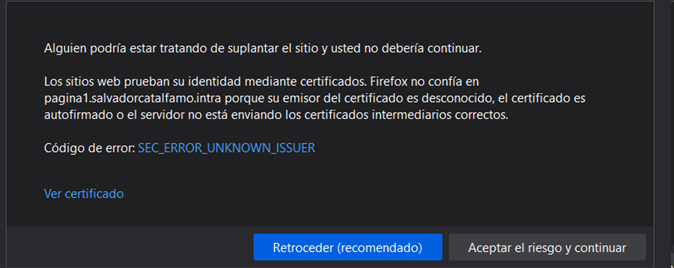
\includegraphics[width=15cm,height=6cm]{adv-2.png}
       \end{center}
       \caption{CA Desconocida}
       \label{figCAdesc}
    \end{figure}
 \end{center}

Luego de establecer en nuestra computadora (particularmente en el navegador Mozilla) que la 
entidad certificante creada es confiable, es posible ver que nuestra conexión es segura, como 
se muestra en la captura.

\begin{center}
    \begin{figure}   
       \begin{center}
          \includegraphics[width=15cm,height=7.5cm]{ca-HTTPS.png}
       \end{center}
       \caption{Resultado de la solución}
    \end{figure}
 \end{center}







Como ventajas de esta propuesta tenemos que no es necesario depender de un 
agente externo para la obtención de certificados, ya que en muchos casos 
no es necesario, y en otros, los certificados provistos por estos no son 
gratuitos. 

Por otro lado, al implementar esta solución, se vio una mayor complejidad 
en la implementación: se requiere un alto entendimiento técnico de todo el 
ciclo de certificación, y un conocimiento sobre las particularidades que 
pueden llegar a existir en la generación de certificados y de llaves privadas. 
Además, hay organizaciones en las que no se tiene el control de todos 
los equipos que se conectan a la red; por ejemplo, empleados externos, 
o bien proveedores de servicios, con lo cual, existe la posibilidad de no 
poder configurar como confiable la entidad certificante en los 
mismos.

Pese a que esta propuesta es de las más implementadas, decidimos buscar 
una opción que nos permita desligarnos de ciertas responsabilidades, 
como así también no tener que realizar configuraciones individuales 
a los hosts de nuestra organización.

\section{Propuesta 3: Certificación con Let's Encrypt}
Esta estrategia consiste en generar un certificado wildcard, y utilizarlo en cada sitio de la organización.
Para esto se debe tener un dominio (en mi caso, salvadorcatalfamo.com) y demostrar la propiedad 
del mismo. Como se vio anteriormente, hay dos maneras que utiliza Let's Encrypt para demostrar la propiedad 
de un dominio, pero la que nos sirve en el caso de una red interna es la que intervienen los registros DNS. 
La verificación que ofrecen con este tipo de certificado es la mínima (DV) y el proceso es explicado a 
continuación.


\subsection{Pasos a seguir}
\subsubsection*{Obtener un dominio}
El primer paso es conseguir un dominio, en mi caso ya tenía uno:
salvadorcatalfamo.com. Este dominio apunta a nuestra ip pública. La configuración DNS
es la siguiente:  


\noindent\begin{minipage}{\textwidth}
   \begin{longtable}{|l|l|p{5cm}|l|l|}
      \hline
      \textbf{Tipo} & \textbf{Nombre} & \textbf{Contenido} & \textbf{Prioridad} & \textbf{TTL}
   \\ \hline A  & salvadorcatalfamo.com & 181.228.121.12 & 0 & 14400
   \\ \hline NS  & salvadorcatalfamo.com & ns1.donweb.com & 0 & 14400
   \\ \hline SOA & salvadorcatalfamo.com & ns2.donweb.com & 0 & 14400
   \\ \hline SOA & salvadorcatalfamo.com & ns3.hostmar.com \newline root.hostmar.com 
                                          \newline 2021010700 28800 7200 
                                          \newline 2000000 86400
                                          \newline ns2.donweb.com & 0 & 14400

                                 
                                          \\ \hline
   \end{longtable}
\end{minipage}

\subsubsection*{Instalando Let’s Encrypt en el servidor}
\begin{verbatim}
   sudo add-apt-repository ppa:certbot/certbotsudo 
   apt-get update
   sudo apt-get install python-certbot-nginx
\end{verbatim}

\subsubsection*{Instalando Nginx}
\begin{verbatim}
sudo apt-get update
sudo apt-get install nginx
\end{verbatim}


\subsubsection*{Obteniendo un certificado SSL de tipo wildcard desde Let’s Encrypt}
\begin{verbatim}
sudo certbot --server https://acme-v02.api.letsencrypt.org/directory 
-d *.salvadorcatalfamo.com --manual --preferred-challenges dns-01 certonly
\end{verbatim}

\subsubsection*{Configuración DNS}
Luego de ejecutar el comando anterior, Let's Encrypt nos da un contenido que 
se debe agregar a un registro DNS. El tipo de registro es TXT y se muestra en
la siguiente tabla.

\begin{longtable}{|l|l|l|l|l|} 
   \hline
   \textbf{Tipo} & \textbf{Nombre} & \textbf{Contenido} & \textbf{Prioridad} & \textbf{TTL}
\\ \hline TXT  & 	\_acme-challenge.salvadorcatalfamo.com & 11UZJD27bPDb\_jFs6f... & 0 & 14400
\\ \hline
\end{longtable}

\subsubsection*{Configuración de Nginx para servir a subdominios}

Se debe modificar el siguiente archivo de 
configuración 

\textit{/etc/nginx/sites-available/salvadorcatalfamo.com} como se muestra a 
continuación:

\begin{verbatim}
server {
   listen 80;
   listen [::]:80;
   server_name *.salvadorcatalfamo.com;
   return 301 https://$host$request_uri;
}
server {
   listen 443 ssl;
   server_name *.example.com;  ssl_certificate /.../.../fullchain.pem;
   ssl_certificate_key /.../privkey.pem;
   include /etc/letsencrypt/options-ssl-nginx.conf;
   ssl_dhparam /.../ssl-dhparams.pem;  root /.../salvadorcatalfamo.com;
   index index.html;
   location / {
      try_files $uri $uri/ =404;
   }
} 
\end{verbatim}


\subsubsection*{Test la configuración y reinicio del servicio}

La configuración se puede testear con el siguiente comando: 
\begin{verbatim}
      sudo nginx -t
\end{verbatim}

Si tiene éxito, se debe volver a cargar Nginx usando
\begin{verbatim}
      sudo /etc/init.d/nginx reload
\end{verbatim}

Ahora Nginx contiene un certificado de tipo wildcard, un certificado SSL con respaldo de una 
entidad certificante como Let's Encrypt

\begin{center}
   \begin{figure}   
      \begin{center}
         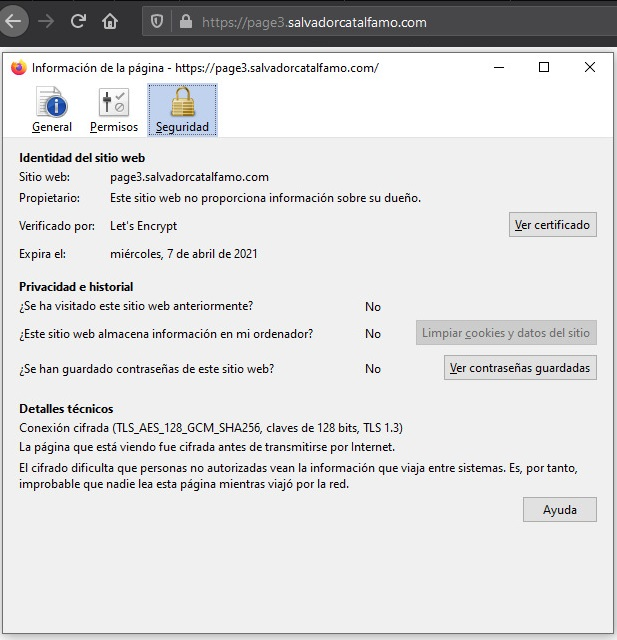
\includegraphics[width=15cm,height=16cm]{lets.png}
      \end{center}
      \caption{Web interna con certificado de Let’s Encrypt}
   \end{figure}
\end{center}

Le hemos visto un gran potencial a esta solución, aunque también es poco implementada. Tenemos la gran ventaja de no
tener que instalar ningún requerimiento en las computadoras dentro de la organización. Con esto, no se 
mostrarán mensajes de seguridad en los navegadores, no importa cuál sea el programa, ya que Let's Encrypt es 
una entidad de confianza para diversos navegadores y sistemas operativos. Todo esto y la seguridad extra al 
saber que nuestros datos van por un canal seguro gracias al protocolo SSL. 

Otra gran ventaja que vimos es la facilidad con la que se llevó a cabo, 
en este proyecto se logró implementar antes esta solución que la entidad certificante, y 
con mucha mayor facilidad. 

Como desventajas podemos decir que no tenemos la posibilidad de obtener la validación extendida (EV), ya que no está
disponible actualmente. Por otro lado, que las llaves privadas y el certificado (que es único para todo el dominio) 
estén en diversos servidores a la vez, implica
que se deben tener mayores recaudos a la hora de utilizarlos, ya que se debe asegurar el control de éstos. Aunque a 
nosotros no nos sucedió, puede llegar a suceder que si se pierde conexión a Internet, el certificado no se pueda validar,
producto de no tener toda la cadena de certificación hasta llegar a la raíz. 

Aunque se puede llegar a pensar, administrar los certificados y las llaves puede llegar a ser 
un gran desafío para los administradores de sistema, sin embargo, hay muchas herramientas que nos proveen
automatización y monitoreo para realizar esta clase de tareas. 


\section{Caso de estudio: Buscando credenciales en tráfico seguro}

Luego de ver las diversas soluciones propuestas, una parte importante de 
nuestro proyecto fue verificar que verdaderamente aumenta la seguridad
cuando nuestro tráfico va encriptado. Para este caso de estudio, se utilizó
el mismo formulario propuesto en la sección \ref{secCaseOfStudy}, lo 
único que con servidores en distintas direcciones.

Dado que el proceso de capturar el tráfico en una red interna fue
explicado previamente, se van a mostrar únicamente los paquetes capturados
desde la primera solicitud hasta el envío del formulario.

\begin{center}
   \begin{figure}   
      \begin{center}
         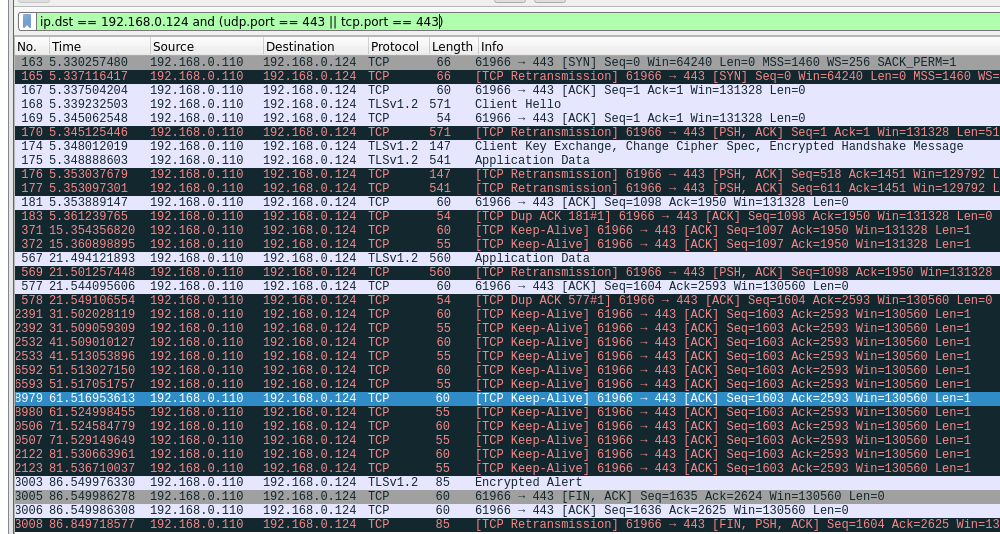
\includegraphics[width=15cm,height=9cm]{verificacion-ssl-1-v2.png}
      \end{center}
      \caption{Tráfico capturado}
   \end{figure}
\end{center}

En esta captura podemos observar que:
\begin{itemize}
   \setlength\itemsep{-0.6em}
   \item No es posible determinar a simple vista cual es el paquete 
   en el cual se envía la información crítica.
   \item Abriendo e investigando el contenido de cada uno de los paquetes mostrados,
   tampoco es posible ver las credenciales completadas en el formulario, 
   que obviamente son de nuestro conocimiento.
   \item Se establece una conexión segura a través del protocolo TCP, algo que no 
   vimos en el caso de estudio de HTTP.
\end{itemize}


